% !TeX root=../main.tex
\chapter{مروری بر مطالعات انجام شده}
%\thispagestyle{empty} 
\section{مقدمه}
در این فصل، پژوهش‌های پیشین در زمینه‌ی موتورهای مسطح مبتنی بر شناوری مغناطیسی (MLPM) با تمرکز بر ویژگی‌های اساسی آنان که به طور کلی در بخش‌های زیر دسته‌بندی شده‌اند، مورد بررسی قرار می‌گیرند. 
\begin{itemize}
	\item
		\textit{معماری دستگاه}:
بررسی انواع معماری‌های موجود برای MLPM و تأثیر آن‌ها بر عملکرد کلی سیستم.
	\item
		\textit{ساختار آهنرباهای دائمی و الکتریکی}:
مرور انواع آهنرباهای الکتریکی و چینش‌های مختلف آهنربا‌های دائمی و نقش آن‌ها در بهینه‌سازی عملکرد سیستم.
	\item
		\textit{طراحی کنترلر}:
معرفی روش‌های کنترل کلاسیک و مدرن برای این سیستم‌ها و چگونگی بهبود پایداری و دقت حرکت.
	\item
		\textit{روش‌های شناسایی سیستم و مدل‌سازی دینامیکی}:
تحلیل روش‌های شناسایی و تخمین مدل‌های دینامیکی سیستم برای شبیه‌سازی و بهینه‌سازی عملکرد.
\end{itemize}
در بخش‌های بعد، پژوهش‌های انجام‌شده بر اساس این ویژگی‌ها ارزیابی شده و مزایا و معایب هر روش مورد بررسی قرار می‌گیرد.

\section{معماری دستگاه‌های MLPM}
سیستم‌های شناوری مغناطیسی به دلیل ماهیت ناپایدارشان بدون استفاده از حلقه‌های کنترلی نمی‌توانند پایداری لازم را فراهم کنند. به همین دلیل، در تمامی ساختارهای پیشنهادی، از سیم‌پیچ‌های الکتریکی برای تولید میدان مغناطیسی با شدت کنترل ‌شده استفاده می‌شود. این سیم‌پیچ‌ها وظیفه دارند تا موقعیت جسم معلق را پایدار کرده و آن را در حالت مطلوب نگه ‌دارند.

در طراحی موتورهای مسطح، که از دو بخش ثابت
\LTRfootnote{Stator}
 و متحرک
\LTRfootnote{Mover}
تشکیل شده‌اند، امکان تغییر در طراحی و محل قرارگیری آهنرباهای الکتریکی و دائمی وجود دارد. نیروی مغناطیسی وارد بر بخش متحرک می‌تواند به‌صورت جاذبه‌ای از بالا یا دافعه‌ای از پایین اعمال شود. با این حال، در موتورهای مسطح به دلیل لزوم کم بودن فاصله میان سیم‌پیچ‌ها و اجسام معلق، اعمال نیروی جاذبه‌ای از بالا امکان‌پذیر نیست. به همین دلیل، در تمامی طراحی‌ها، نیروی مغناطیسی دافعه‌ای از سمت پایین به بخش متحرک وارد می‌شود که امکان جابه‌جایی اجسامی که بر روی آنها قرار می‌گیرند را فراهم می‌کند.

با توجه به این موارد، دو طراحی کلی برای ساخت دستگاه‌های MLPM ارائه می‌شود که در ادامه بررسی می‌‌شوند.
\subsection{سیم‌پیچ‌های متحرک و آهنرباهای ثابت}

در این معماری، بخش استاتور از مجموعه‌ای آهنربای ثابت تشکیل شده که میدان مغناطیسی پایدار در محیط اطراف خود ایجاد می‌کنند. بخش متحرک دستگاه شامل سیم‌پیچ‌هایی است که با عبور جریان الکتریکی از آن‌ها، میدان مغناطیسی متغیری تولید می‌گردد. این جریان به گونه‌ای تنظیم می‌شود که نیروی وارد بر آهنرباهای دائمی به‌دقت کنترل شود. طبق قانون سوم نیوتن، نیروهای وارد بر سیم‌پیچ‌ها و آهنرباهای دائمی به‌عنوان عمل و عکس‌العمل رفتار می‌کنند؛ به این ترتیب، نیرویی که به آهنرباها اعمال می‌شود، باعث ایجاد نیرویی برابر و در جهت مخالف بر سیم‌پیچ‌ها خواهد شد.

در پژوهش 
\cite{RN49}
، از ساختاری با سیم‌پیچ‌های چندلایه متعامد در بخش متحرک استفاده شده است. لایه اول سیم‌پیچ‌ها نیرویی را در راستاهای x و z ایجاد می‌کند، در حالی که لایه دوم نیرو را در راستاهای y و z اعمال می‌کند. این جداسازی نیروها به بهبود کنترل سیستم کمک می‌کند. علاوه بر این، به دلیل تفاوت فاصله میان لایه‌ها و استاتور، نیروهای تولیدشده توسط هر لایه متفاوت خواهند بود. راهکار ارائه‌شده برای این چالش، افزایش ضخامت لایه‌های دورتر از استاتور است. با این حال، برای جلوگیری از مشکلات ناشی از تفاوت ضخامت لایه‌ها، ساختاری سه‌لایه طراحی شده که ضمن افزایش نیروی تولیدی، ضخامت یکنواختی را در تمامی راستاها فراهم می‌نماید. در شکل 
\ref{fig:Multilayer_Mover_Coil}
ساختار این دستگاه نمایش داده شده است.

در پژوهش 
\cite{RN38}
، بخش متحرک از یک لایه سیم‌پیچ با چینش متعامد تشکیل شده که قابلیت اعمال نیرو در سه راستا را فراهم می‌سازد. در ادامه، پژوهش
\cite{RN14}
 روشی تحلیلی برای بهینه‌سازی ضخامت این سیم‌پیچ‌ها ارائه کرده است که با در نظر گرفتن معیارهای مختلف، به بهبود عملکرد سیستم می‌پردازد. شکل 
\ref{fig:Single_layer_Mover_Coil}
 این ساختار را نمایش داده است.

\begin{figure}[ht]
\centering 
\subfloat[استفاده از سیم‌پیچ‌های چندلایه
\cite{RN49}]
{ \label{fig:Multilayer_Mover_Coil}
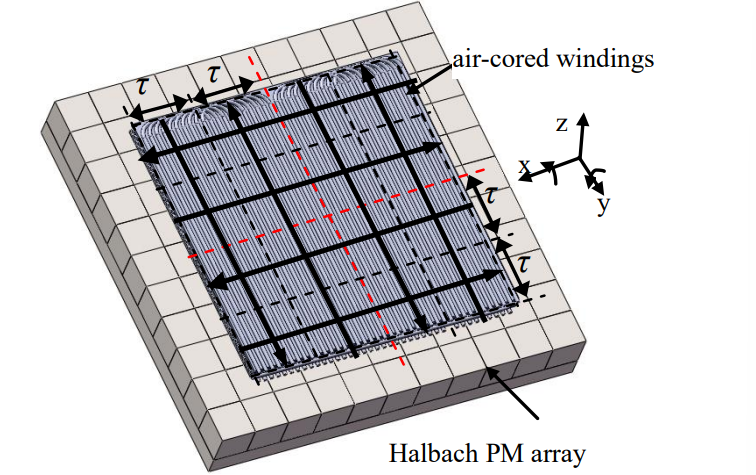
\includegraphics[width=0.5\textwidth]{Multilayer_Mover_Coil}}
%\hspace{2mm}
\subfloat[استفاده از سیم‌پیچ‌های یک لایه متعامد
\cite{RN14}]
{ \label{fig:Single_layer_Mover_Coil}
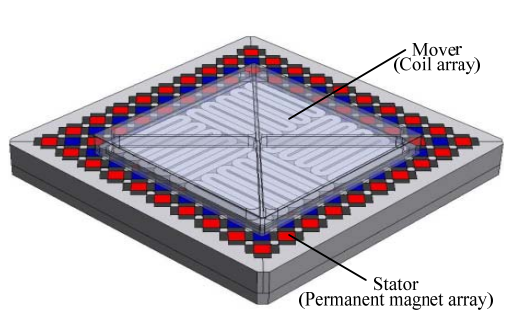
\includegraphics[width=0.5\textwidth]{Single_layer_Mover_Coil}}%
\caption{ساختار سیستم‌های MLPM با سیم‌پیچ‌های متحرک و آهنربای ثابت}
\label{fig:Moveing_Coil} %% label for entire figure
\end{figure}

با وجود اینکه این معماری امکان دستیابی به شناوری پایدار و حرکت با شش درجه آزادی را فراهم می‌کند، اما در کاربردهای عملی با محدودیت‌هایی مواجه است که بر عملکرد نهایی سیستم تأثیرگذار هستند. نخستین محدودیت، نیاز به تأمین انرژی الکتریکی برای سیم‌پیچ‌ها از طریق سیم‌های فیزیکی است که این امر به‌طور اجتناب‌ناپذیری ارتباط فیزیکی میان جسم متحرک و محیط اطراف را برقرار می‌سازد، در نتیجه حرکت آزادانه کامل جسم متحرک محدود می‌شود. دومین محدودیت، چالش خنک‌کاری سیم‌پیچ‌ها است که به دلیل ماهیت متحرک و معلق بودن آن‌ها، اجرای یک سیستم خنک‌کننده کارآمد دشوار خواهد بود. این مشکلات، نیاز به ارائه معماری جدیدی را آشکار می‌کند که بتواند این چالش‌ها را برطرف سازد.

\subsection{‌آهنرباهای متحرک و سیم‌پیچ‌های ثابت}

معماری دیگری که برای طراحی دستگاه‌های MLPM ارائه شده است، شامل قرار دادن سیم‌پیچ‌ها در بخش استاتور و استفاده از آهنرباهای دائمی در بخش متحرک می‌باشد. این ساختار نوین که در بسیاری از پژوهش‌ها مورد استفاده قرار گرفته، مشکلات معماری‌های پیشین مانند محدودیت جابه‌جایی متحرک ناشی از اتصالات فیزیکی و چالش‌های خنک‌کاری سیم‌پیچ‌ها را برطرف کرده و منجر به بهبود عملکرد کلی سیستم شده است.

در پژوهش 
\cite{RN7}
 استاتوری با چینش سیم‌پیچ‌ها مطابق با الگوی شاه‌ماهی
\LTRfootnote{Herringbone pattern}
 طراحی و پیاده‌سازی شده است. این طراحی امکان اعمال نیروی مغناطیسی به دو آهنربای دیسکی تعبیه‌شده در بخش متحرک را فراهم کرده است که دقتی در حدود 1 درجه در زوایای حرکت و 1 میلی‌متر در موقعیت متحرک به دست آورده است
\cite{RN7}
. در ادامه این پژوهش، ساختاری جدید برای بخش متحرک ارائه شده که شامل 6 آهنربای دیسکی با چینش کروی و فواصل ثابت می‌باشد. این طراحی توانسته است چرخش آزادانه متحرک را حول سه محور ممکن سازد 
\cite{RN39}.
شکل (
\ref{fig:Moving_Magnet_1})
همچنین در پژوهش 
\cite{RN62}
 نیز از این چینش سیم‌پیچ‌ها استفاده شده و مطابق با شبیه‌سازی‌های ارائه شده، مزیت آنان در ایجاد میدان مغناطیسی یکنواخت‌تر در نواحی کناری سیم‌پیچ‌ها نمایش داده شده است.

استفاده از سیم‌پیچ‌های سه‌فاز به‌جای تغذیه با جریان مستقیم، رویکردی است که در پژوهش 
\cite{RN24}
معرفی و اجرا شده است. در این ساختار، چهار آرایه از سیم‌پیچ‌های سه‌فاز، همان‌طور که در 
شکل (
\ref{fig:Moving_Magnet_2})
 نشان داده شده است، به‌گونه‌ای طراحی شده‌اند که نیروی مغناطیسی لازم را تولید کنند.

به ‌منظور کاهش هزینه‌ی محاسباتی در جابه‌جایی‌های طولانی، پژوهش 
\cite{RN32}
 ساختاری را ارائه کرده است که از دو مجموعه سیم‌پیچ‌ سه‌فاز و تک‌فاز تشکیل شده است. در این طراحی، کنترل حرکت در مسافت‌های طولانی توسط سیم‌پیچ‌های سه‌فاز انجام می‌پذیرد، در حالی که برای تنظیم دقیق موقعیت متحرک در صفحه، از سیم‌پیچ‌های تک‌فاز بهره برده می‌شود.
شکل (
\ref{fig:Moving_Magnet_3})

استفاده از سیم‌پیچ‌های ماژولار در طراحی استاتورهایی با چینش دوبعدی، رویکردی است که در دستگاه‌های MagTable و MagFloor از دانشگاه واترلو پیاده‌سازی شده است
\cite{RN8,RN30,RN10}
 در این طراحی، ماژول‌هایی از سیم‌پیچ‌های با سطح مقطع مربع به‌گونه‌ای طراحی شده‌اند که با قرار گرفتن در کنار یکدیگر، فضای کاری نامحدودی برای جابه‌جایی متحرک فراهم می‌کنند.(شکل
\ref{fig:Moving_Magnet_4})
 همچنین، پژوهش
\cite{RN8}
 نشان داده است که آهنرباهای با سطح مقطع مربع، در مقایسه با سیم‌پیچ‌های دایروی با جریان الکتریکی مشابه، می‌توانند شدت میدان مغناطیسی بیشتری ایجاد کنند، که این مزیت عملکرد کلی سیستم را بهبود می‌بخشد.

\begin{figure}[ht]
\centering 
\subfloat[الگوی شاه‌ماهی سیم‌پیچ‌ها
\cite{RN39}]
{ \label{fig:Moving_Magnet_1}
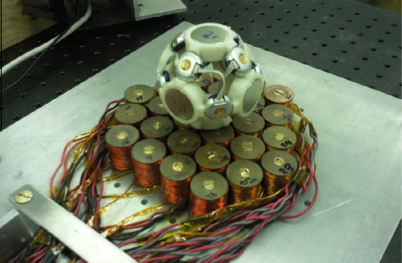
\includegraphics[width=0.45\textwidth]{Moving_Magnet_1}}
\hspace{2mm}
\subfloat[سیم‌پیچ‌های سه فاز
\cite{RN24}]
{ \label{fig:Moving_Magnet_2}
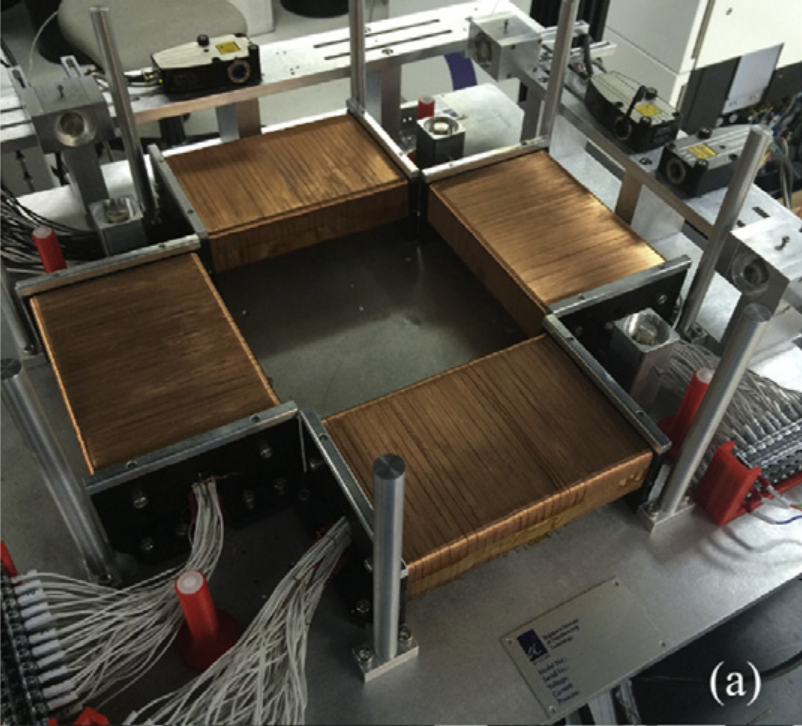
\includegraphics[width=0.45\textwidth]{Moving_Magnet_2}}
\\ % Newline to wrap the figures to the next row
\subfloat[ساختار دوگانه سیم‌پیچ‌ها
\cite{RN32}]
{ \label{fig:Moving_Magnet_3}
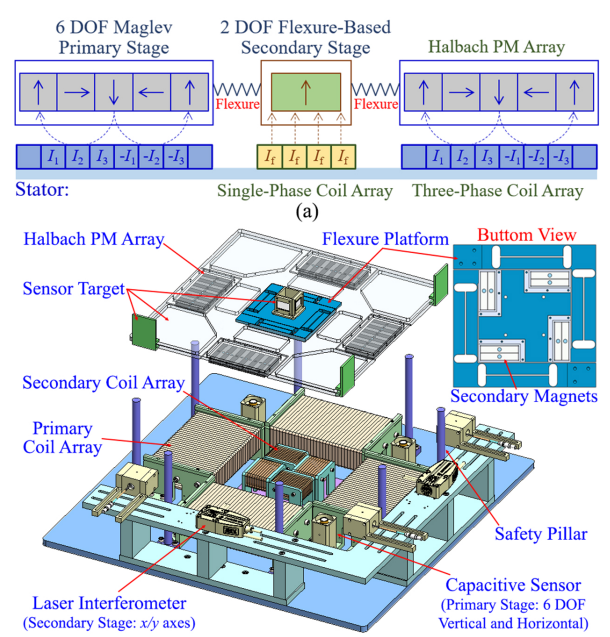
\includegraphics[width=0.45\textwidth]{Moving_Magnet_3}}
\hspace{2mm}
\subfloat[ساختار ماژولار سیم‌پیچ‌ها
\cite{RN10}]
{ \label{fig:Moving_Magnet_4}
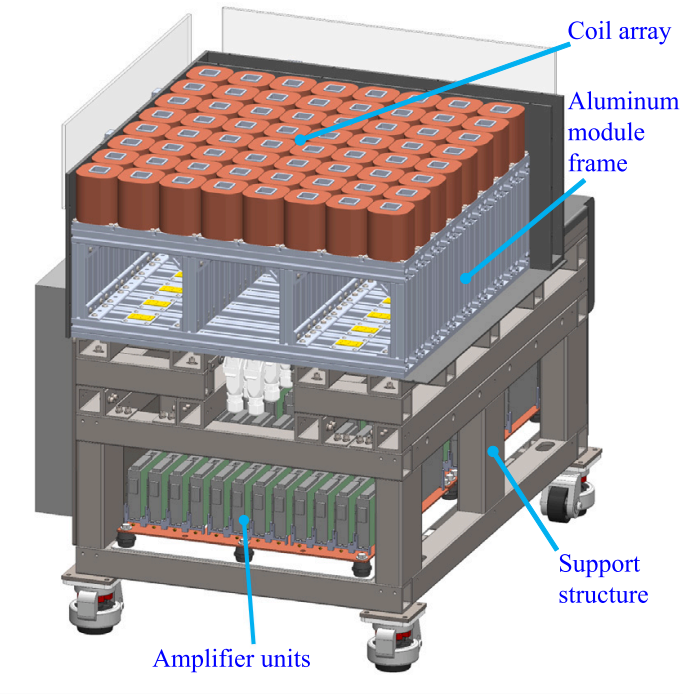
\includegraphics[width=0.45\textwidth]{Moving_Magnet_4}}
\label{fig:Moveing_Magnet} %% label for entire figure
\caption{ساختارهای آهنرباهای متحرک و سیم‌پیچ‌های ثابت}
\end{figure}








\section{ساختار آهنرباهای دائمی}

همان‌طور که در بخش قبل اشاره شد، میدان مغناطیسی کنترل‌شده توسط آهنرباهای الکتریکی ایجاد می‌شود و بر اثر تعامل این میدان متغیر با میدان ثابت آهنرباهای دائمی، نیرویی بر بخش متحرک دستگاه وارد می‌شود که حرکت آن را در راستاهای مختلف ممکن می‌سازد. بنابراین، طراحی بهینه آهنرباهای دائمی، به‌ویژه برای تولید میدان مغناطیسی قوی‌تر با کمترین وزن، در بهبود کارایی دستگاه نقش کلیدی دارد. در این بخش، طراحی‌های مختلف آهنرباهای دائمی که در پژوهش‌های پیشین ارائه شده‌اند، با تمرکز بر بهینه‌سازی این ویژگی‌ها بررسی می‌شوند.
\subsection{استفاده از آهنرباهای دیسکی}

استفاده از آهنرباهای دیسکی رویکردی ساده و مؤثر برای ایجاد میدان مغناطیسی دائمی محسوب می‌شود. با انتخاب موادی با خاصیت مغناطیسی بالا، مانند آهنرباهای نئودیمیومی، می‌توان به شدت میدان مغناطیسی مطلوب دست یافت. به عنوان نمونه، در پژوهش 
\cite{RN7}
 از دو آهنربای دیسکی جهت تأمین میدان مغناطیسی ثابت استفاده شده است. همچنین در پژوهش 
\cite{RN39}
 با به‌کارگیری ۶ آهنربای دیسکی، امکان چرخش آزادانه حول سه محور فراهم شده است.(شکل
\ref{fig:Disk_Magnet_1})
 در پژوهش 
\cite{RN8}
 نیز از ترکیب‌های متفاوتی از آهنرباهای دیسکی برای بخش متحرک دستگاه استفاده شده است، که این ترکیب‌ها شامل تغییر اندازه‌ی یک آهنربا و استفاده از سه آهنربای دیسکی است. سیستم شناوری مغناطیسی با پنج درجه آزادی که تنها از یک آهنربای دیسکی تشکیل شده است، در پژوهش 
\cite{RN62}
 به عنوان نمونه‌ای موفق از این رویکرد معرفی شده است. این طراحی، با وجود سادگی معماری، توانسته نتایج رضایت‌بخشی را از نظر عملکرد ارائه دهد و نشان می‌دهد که استفاده از آهنربای دیسکی، علاوه بر سادگی، می‌تواند در کاربردهای مختلف به‌ویژه در سیستم‌های با نیاز به دقت بالا و چند درجه آزادی، کارآمد باشد. شکل((
\ref{fig:Disk_Magnet_2})


\begin{figure}[ht]
\centering 
\subfloat[دو آهنربای دیسکی
\cite{RN7}]
{ \label{fig:Disk_Magnet_1}
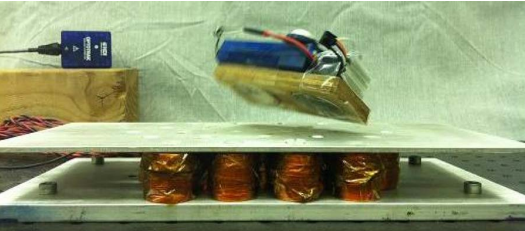
\includegraphics[width=0.5\textwidth]{Disk_Magnet_1}}
%\hspace{2mm}
\subfloat[یک آهنربای دیسکی
\cite{RN62}]
{ \label{fig:Disk_Magnet_2}
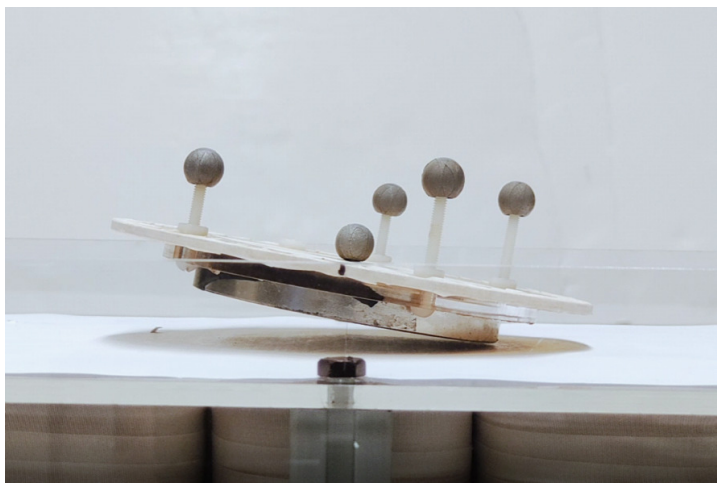
\includegraphics[width=0.5\textwidth]{Disk_Magnet_2}}%
\caption{استفاده از آهنربای دیسکی در طراحی متحرک}
\label{fig:Disk_Magnet} %% label for entire figure
\end{figure}



\subsection{آرایه‌ی هالباخ یک بعدی}

آرایه‌ی هالباخ
\LTRfootnote{Halbach Array}
 به‌عنوان چینشی از آهنرباهای دائمی تعریف می‌شود که در آن جهت مغناطیس‌شوندگی هر آهنربا با آهنربای مجاور خود ۹۰ درجه تفاوت دارد. این آرایه به‌طور خاص قادر است میدان مغناطیسی در یک سوی آرایه را خنثی کرده و در سوی دیگر میدان را به میزان تقریبی ۱.۴ برابر افزایش دهد.
مزیت این ساختار در طراحی سیستم‌های MLPM، توانایی آن در تولید شدت میدان مغناطیسی بیشتر است. به‌همین‌دلیل، این چینش در بسیاری از پژوهش‌ها مورد استفاده قرار گرفته است.
با این حال، استفاده از تنها یک آرایه‌ی یک‌بعدی هالباخ به‌تنهایی نمی‌تواند نیرویی در دو راستای افقی ایجاد کند. لذا معمولاً از تعداد بیشتری از این آرایه‌ها در ساختار متحرک استفاده می‌شود. به‌عنوان مثال، در پژوهش‌های 
\cite{RN24,RN27}
 از چهار آرایه‌ی هالباخ یک‌بعدی در بخش متحرک استفاده شده است که هر یک از این آرایه‌ها قادر به ایجاد نیرویی در یکی از راستاهای افقی و عمودی هستند.
در پژوهش 
\cite{RN39}
، مشابه آنچه که در بخش استاتور پیاده‌سازی شده بود، از ساختار دوگانه‌ای در بخش متحرک بهره‌برداری شده است، به‌گونه‌ای که دو مجموعه چهارگانه از آرایه‌های هالباخ در معماری این بخش به‌کار رفته‌اند.

\begin{figure}[ht]
\centering 
\subfloat[آرایه‌ی هالباخ
\cite{RN16}]
{ \label{fig:halbach1D}
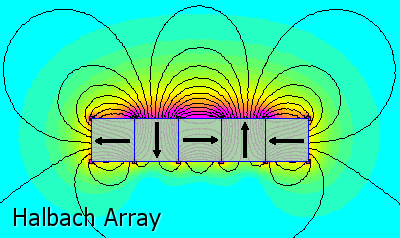
\includegraphics[width=0.5\textwidth]{halbach1D}}
%\hspace{2mm}
\subfloat[4 آرایه‌ی یک بعدی هالباخ
\cite{RN39}]
{ \label{fig:4_halbach1D_array}
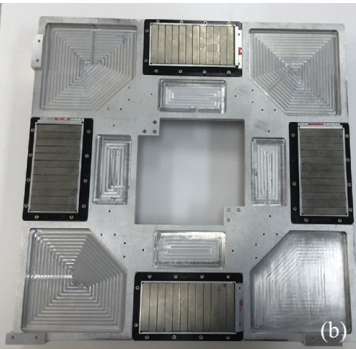
\includegraphics[width=0.5\textwidth]{4_halbach1D_array}}%
\caption{آرایه هالباخ یک‌بعدی}
\label{fig:halbach1D} %% label for entire figure
\end{figure}

\subsection{آرایه هالباخ دوبعدی}

برای رفع محدودیت‌های آرایه‌ی هالباخ یک‌بعدی که تنها در یک راستا نیرو ایجاد می‌کند، ساختار جدیدی از آرایه‌ی دوبعدی ارائه شده است. این آرایه قادر است میدان مغناطیسی را در یک طرف صفحه حذف و در طرف دیگر تقویت کند. با این ویژگی، استفاده از چندین آرایه برای تأمین میدان مغناطیسی ثابت ضروری نخواهد بود. طراحی آرایه‌ی دوبعدی در بسیاری از پژوهش‌ها برای بخش‌های متحرک یا استاتور سیستم‌های MLPM به کار گرفته شده است.

استفاده از آرایه‌ی هالباخ در پژوهش‌های مختلفی از جمله
\cite{RN10, RN30} 
و
\cite{RN55, RN26} 
نشان‌دهنده‌ی عملکرد بهینه‌ی این معماری در بخش متحرک سیستم‌های MLPM است.(شکل
\ref{fig:halbach2D_2})
 همچنین در پژوهش
\cite{RN14}
 از این آرایه به عنوان بخشی از استاتور دستگاه بهره‌گیری شده است. در 
\cite{RN61}
 ماژول‌هایی برای ساخت این آرایه استفاده شده (شکل
\ref{fig:halbach2D_4})
 و در
\cite{RN49}
 برای تشکیل آرایه از قطعات آهنی در فضای خالی میان آن استفاده شده است؛ اما این رویکرد باعث ایجاد خطا در دقت میدان مغناطیسی شده است. (شکل
\ref{fig:halbach2D_3})
علاوه بر این، در پژوهش
\cite{RN28}
، طراحی جدیدی با آهنرباهایی با میزان مغناطیس‌شوندگی و ارتفاع متفاوت پیشنهاد شده است.

\begin{figure}[ht]
\centering 
\subfloat[آرایه هالباخ دو بعدی و میدان مغناطیسی آن
\cite{RN10}]
{ \label{fig:halbach2D_2}
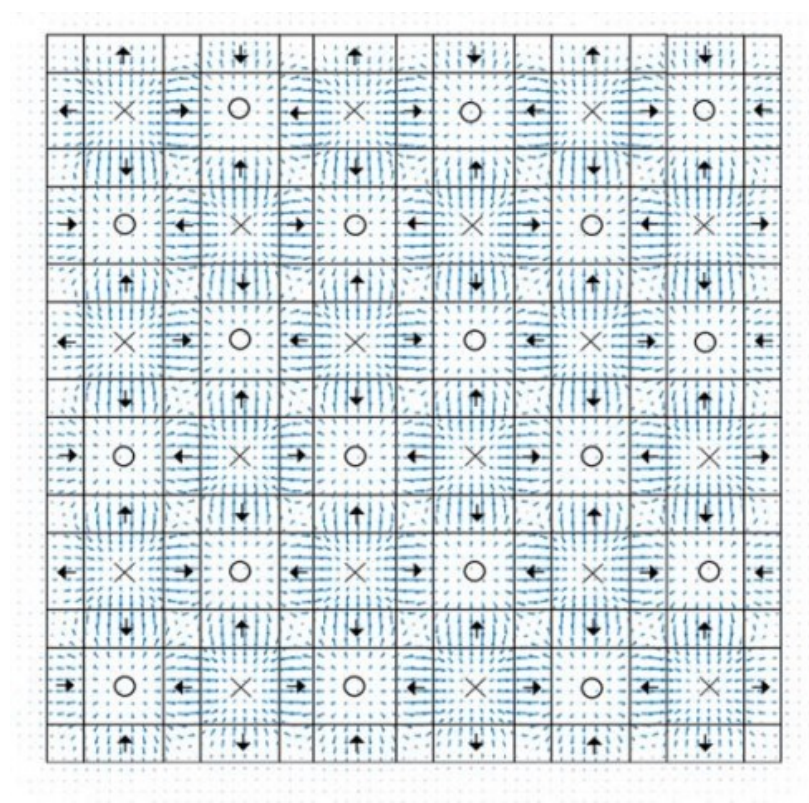
\includegraphics[width=0.45\textwidth]{halbach2D_2}}
\hspace{2mm}
\subfloat[آرایه هالباخ دوبعدی با قطعات آهنی در فضاهای خالی
\cite{RN49}]
{ \label{fig:halbach2D_3}
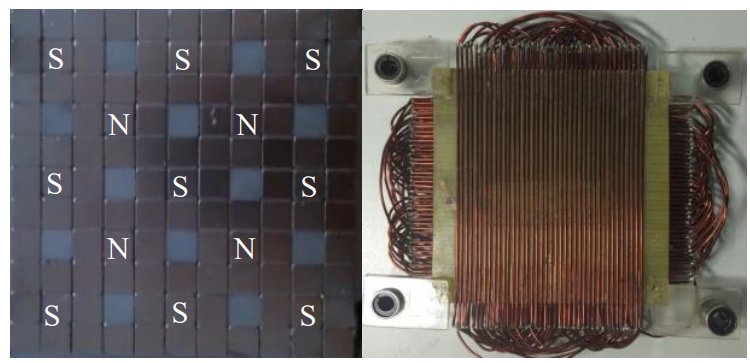
\includegraphics[width=0.45\textwidth]{halbach2D_3}}
\\ % Newline to wrap the figures to the next row
\subfloat[آرایه هالباخ دوبعدی ماژولار
\cite{RN61}]
{ \label{fig:halbach2D_4}
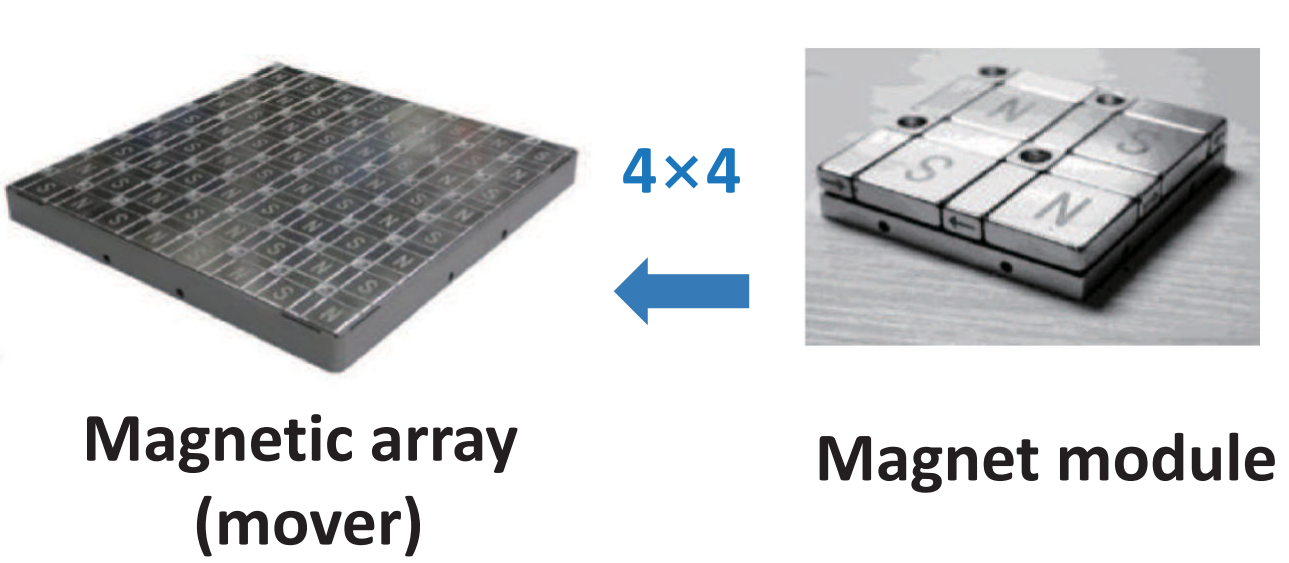
\includegraphics[width=0.45\textwidth]{halbach2D_4}}
\caption{آرایه هالباخ دو‌بعدی}
\label{fig:halbach2D} %% label for entire figure

\end{figure}

































